El presente Trabajo de Fin de Grado documenta el proceso de diseño y desarrollo de Reset, un videojuego en 2.5D de estética Pixel Art que explora y aúna diferentes géneros clásicos bajo una misma experiencia narrativa. En este primer capítulo se establecen las bases conceptuales del proyecto, exponiendo el contexto actual de la industria y las motivaciones principales que impulsan el desarrollo; analizando el estado del arte de los géneros y correspondientes subgéneros implementados y, finalmente, se detallan los objetivos generales y específicos que guían este trabajo.


\subsection{Contexto del Proyecto}

El proyecto \textit{Reset} nace de la voluntad de integrar y sintetizar el conjunto de competencias y conocimientos técnicos adquiridos a lo largo del Grado Universitario. Desde una perspectiva de ingeniería del software y diseño de interacciones, el núcleo conceptual del juego reside en la \textbf{unificación de géneros discordantes dentro de una misma arquitectura de software}.

La motivación principal de este proyecto radica en el deseo de no limitar un trabajo de esta relevancia a un único ámbito del diseño y desarrollo de videojuegos. Por el contrario, se persigue un desarrollo global y transversal que permita plasmar las competencias y conocimientos adquiridos a lo largo del grado en todas sus dimensiones. Esta meta de carácter académico se unifica con una motivación de índole personal: concebir una obra cuyo trasfondo rinda homenaje a los títulos de referencia que han marcado la trayectoria del autor como jugador y que, en última instancia, despertaron su vocación por esta disciplina. En definitiva, el proyecto busca establecer una sinergia entre el rigor técnico y conceptual exigido en el ámbito universitario y el tributo creativo a las obras que inspiraron el inicio de esta formación.

Asimismo, dado que el perfil profesional del autor no se limita exclusivamente al desarrollo técnico, sino que abarca un gran interés por áreas como el diseño visual y jugable o la interfaz y experiencia de usuario (UI/UX) y la animación, se optó por abordar el proyecto desde una perspectiva multidisciplinar. De este modo, la implementación de la arquitectura de software y los sistemas de programación se complementa de forma equilibrada con un riguroso trabajo en el apartado visual y de interacción, buscando un acabado final pulido que ponga en valor ambas facetas de la creación de videojuegos.

Por ello, en lugar de desarrollar un videojuego limitado a un único bucle de juego básico (\textit{core gameplay loop}), \textit{Reset} se diseña como una plataforma experimental que transiciona dinámicamente entre la perspectiva cenital (\textit{Top-Down}) orientada a la acción y la supervivencia táctica, y la perspectiva lateral (\textit{Side-Scroller}) orientada al plataformeo clásico y de precisión. Este enfoque plantea un desafío técnico directo: la creación de un sistema modular unificado capaz de gestionar físicas, inventarios y estados de juego completamente heterogéneos entre mundos, garantizando una experiencia de usuario fluida y coherente.

\subsection{El panorama actual y la barrera de entrada a los géneros}

La industria del videojuego ha evolucionado exponencialmente en las últimas décadas, diversificándose en una inmensa cantidad de géneros y subgéneros. Si bien esta variedad enriquece el medio, también genera un efecto de 'zonas de confort' entre los jugadores habituales, quienes tienden a consumir reiteradamente un mismo tipo de género (como los shooters, los juegos de rol o los títulos deportivos).

A este fenómeno se suma la propia evolución del desarrollo y la aparición de nuevos estudios de forma creciente año tras año, lo que ha provocado un incremento masivo en la publicación anual de títulos en comparación a periodos anteriores. Esta sobresaturación del mercado refuerza el aislamiento del jugador; al disponer de una oferta prácticamente inabarcable de su género favorito, el usuario tiende a especializarse. Inevitablemente, acaba convirtiéndose en un jugador de ``nicho'' que dedica todo su tiempo de ocio a iterar sobre las mecánicas que ya domina y disfruta, en lugar de abrir sus posibilidades a nuevas experiencias fuera de esa zona de confort o a recordar dinámicas y géneros que anteriormente disfrutaba.

Es en este contexto donde nace la motivación principal de \textit{Reset}. El proyecto se concibe con la ambición de abarcar al mayor número de perfiles de jugador posible, actuando como un puente estratégico. Para los jugadores de nicho, el título utiliza sus géneros predilectos como gancho inicial para captar su atención y, progresivamente, animarles a transicionar hacia mecánicas desconocidas.

Simultáneamente, \textit{Reset} sirve como puerta de entrada para usuarios con poca experiencia, ofreciéndoles una cata interactiva donde pueden experimentar con diversos géneros y subgéneros. Para lograr este acercamiento bidireccional, el proyecto se apoya en la narrativa como ancla emocional, logrando que los jugadores menos experimentados empaticen con la historia y mantengan su atención mientras descubren sus propios gustos sin la fricción de tener que adquirir y aprender a jugar múltiples títulos independientes.

\subsection{El reto del diseño: Cohesión frente a fragmentación}

Al plantear un videojuego que combine múltiples géneros, el mayor riesgo en la fase de diseño era caer en la creación de una simple ``colección de minijuegos'' inconexos. A nivel personal y profesional, el objetivo primordial era deconstruir esa estructura fragmentada para construir una experiencia verdaderamente lineal y cohesiva.

Para lograr que los jugadores no sintieran estos saltos de género como una ruptura del \textit{game feel}, era imperativo diseñar un hilo conductor lo suficientemente robusto. La solución adoptada fue dotar al proyecto de una narrativa profunda y emocional que justificara, de manera orgánica dentro del propio universo del juego, cada cambio de perspectiva, física y control.

De la misma forma, esta narrativa serviría como gancho para los jugadores principiantes. Al tratarse de mecánicas, perspectivas y ambientaciones completamente diferentes en cada nivel, el usuario podría perderse o frustrarse al encontrarse con un género que quizás no logre captar toda su atención. Es en ese momento donde la narrativa rescata la percepción de este tipo de jugador, ayudándole a progresar con el fin general de completar una historia con la que previamente haya conectado.

\subsection{El reto de jugabilidad: Imposibilidad frente a aburrimiento}

Aglutinar a un público tan dispar (—)desde el jugador de nicho altamente experimentado hasta el usuario novato) plantea un desafío de diseño crítico: el balanceo de la dificultad. Basándose en la teoría de flujo\cite{csikszentmihalyi1990flow}, si un nivel es demasiado exigente, el jugador inexperto chocará contra un muro de imposibilidad y abandonará el juego por frustración; por el contrario, si el reto es excesivamente simple, el jugador veterano caerá en el aburrimiento.

Para resolver esta dicotomía en \textit{Reset}, se ha optado por un diseño de niveles estructurado en capas. La ruta principal de cada mundo está diseñada para ser un reto accesible con su dedicada curva de aprendizaje, donde las métricas de física y la agresividad de los enemigos permiten un avance fluido con un amplio margen de error. Esto garantiza que cualquier jugador pueda disfrutar de la transición de géneros y avanzar en la historia. Sin embargo, para satisfacer a los jugadores más experimentados que buscan exprimir al máximo el rendimiento y las mecánicas, se integran rutas secundarias y desafíos opcionales. Estas bifurcaciones elevan drásticamente el nivel de exigencia, premiando la maestría y la precisión sin penalizar el progreso general del resto de usuarios.


\section{Estado del arte}

El diseño y desarrollo de un videojuego multigénero requiere una comprensión profunda de las convenciones, mecánicas y la evolución histórica de los estilos que busca unificar. Para contextualizar adecuadamente el enfoque y las decisiones de diseño tomadas en \textit{Reset}, se analiza el contexto de evolución de los géneros de videojuegos, los cuales con el paso del tiempo han derivado en una enorme diversificación, así como el estado del arte de las dos grandes corrientes lúdicas que conforman el núcleo de este prototipo funcional (\textit{Vertical Slice}): la aventura de acción con tintes de supervivencia en perspectiva cenital (\textit{Top-Down}) y el género de plataformas bidimensional (\textit{Side-Scrolling}), abarcando tanto su vertiente más clásica como el plataformas de precisión moderno.

A través de este análisis, se explorarán las obras referentes que sentaron las bases fundacionales de los videojuegos hasta derivar en ambos paradigmas mencionados, cómo han evolucionado sus mecánicas principales a lo largo de las décadas y de qué manera sus filosofías de diseño influyen en la actualidad. Comprender este recorrido histórico es un paso fundamental para justificar las resoluciones arquitectónicas y jugables implementadas durante el desarrollo de este proyecto. De este modo, se explican la integración de mecánicas dispares entre niveles, unificadas bajo un mismo motor y una estética cohesionada, representando un estudio técnico y práctico de la propia historia del medio interactivo.

\subsection{El origen y la diversificación de los géneros en el videojuego}

En los comienzos de la industria de los videojuegos, las limitaciones tecnológicas dictaban de forma absoluta el diseño de las experiencias jugables. Durante la década de los setenta y principios de los ochenta, el nacimiento de los videojuegos estuvo íntimamente ligado a los salones recreativos. En este contexto emergió el género Arcade, caracterizado por mecánicas directas, partidas de muy corta duración y una curva de dificultad extremadamente pronunciada. Su diseño no buscaba la inmersión a largo plazo, sino incentivar al jugador a intentar una y otra vez superar una puntuación o nivel con el fin de hacerle gastar más monedas en la misma máquina recreativa. Títulos como \textit{Space Invaders} (1978)\cite{space_invaders_game} o \textit{Pac-Man} (1980)\cite{pacman_game} (ver Figura~\ref{fig:SpacePacMan}) sentaron las bases de la interacción digital, pero limitaban su alcance a la superación de puntuaciones en pantallas estáticas o con un desplazamiento bidimensional muy rudimentario.

Sin embargo, la llegada y democratización de las consolas domésticas de 8 y 16 bits como la NES de Nintendo (ver Figura~\ref{fig:NintendoNES}) o la Mega Drive de SEGA, supuso un cambio de paradigma radical. Aunque la transición al salón del hogar se inició previamente con el lanzamiento de la \textit{Magnavox Odyssey} (1972), esta primera etapa aún heredaba el modelo de diseño y consumo efímero del entorno arcade. Fue con el desembarco de las plataformas japonesas cuando los desarrolladores se liberaron de la necesidad de diseñar en torno a la monetización rápida, permitiendo concebir partidas de larga duración. La introducción de sistemas de guardado en la memoria (inicialmente mediante contraseñas y posteriormente a través de pilas internas en los propios cartuchos) fue el catalizador definitivo para la diversificación y explosión de los géneros. Al dotar a los juegos de memoria, se abría la puerta al progreso continuado y a la narrativa extensa, dando lugar a títulos con una línea de progresión clara, un inicio definido y un desenlace.

\begin{figure}[htbp]
    \centering
    % Subfigura izquierda (Space Invaders)
    \begin{subfigure}[b]{0.45\textwidth}
        \centering
        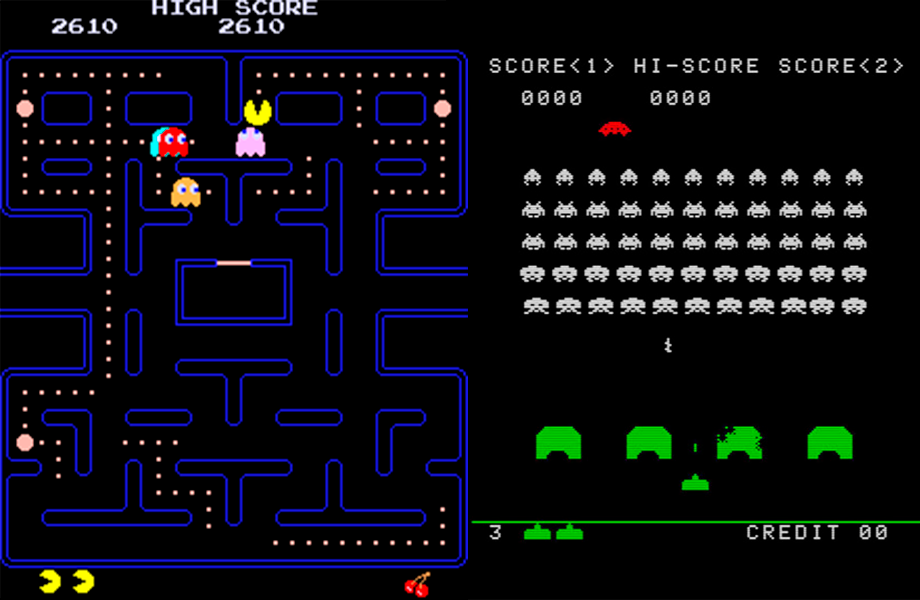
\includegraphics[width=\textwidth]{pages/img/Arcades.png}
        \caption{Pantallas de juego de \textit{Space Invaders} (1978) y \textit{Pac-Man} (1980).}
        \label{fig:SpacePacMan}
    \end{subfigure}
    \hfill
    % Subfigura derecha (Pac-Man)
    \begin{subfigure}[b]{0.45\textwidth}
        \centering
        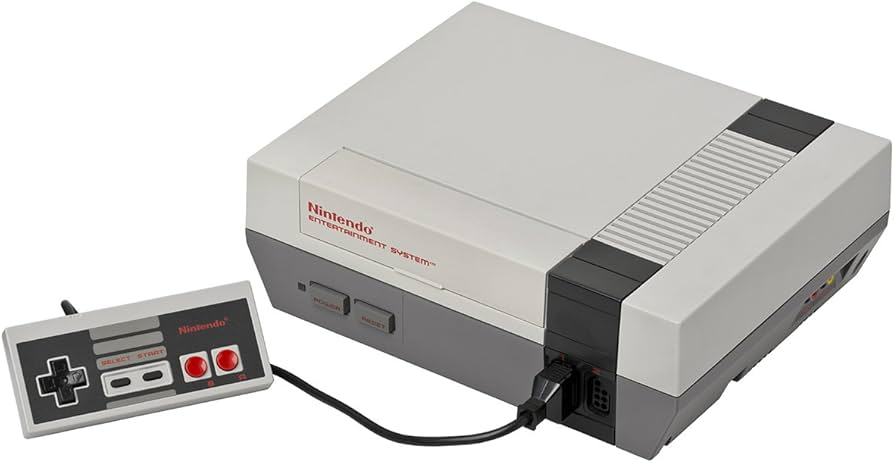
\includegraphics[width=\textwidth]{pages/img/NES.jpg}
        \caption{Nintendo NES original (1985).}
        \label{fig:NintendoNES}
    \end{subfigure}
    \caption{Títulos pioneros orientados a la superación de puntuaciones en la época arcade.}
    \label{fig:Contexto1}
\end{figure}

Es en esta etapa histórica es donde se consolidan las grandes corrientes lúdicas que cimentaron las bases de la industria actual y que sirven de referente directo para este proyecto:

\begin{itemize}
    \item \textbf{Juegos de Acción y Plataformas:} Evolucionaron desde el formato de salto en una pantalla estática hacia el desplazamiento lateral continuo (\textit{Side-Scrolling}). Se priorizó la habilidad rítmica, el control de la inercia y la superación de obstáculos físicos, convirtiéndose en el género estandarte de las consolas de 8 y 16 bits gracias a referentes como \textit{Super Mario Bros.} (1985)\cite{mario_bros_game} o \textit{Sonic the Hedgehog} (1991)\cite{sonic_game} (ver Figura~\ref{fig:plataformas}). El primero supuso uno de los grandes puntos de inflexión en la concepción lúdica de los ochenta, ya que fue de los primeros títulos en trasladar el estilo arcade a la unificación narrativa. Con ello, dotó al juego de un ciclo cohesivo mediante una travesía estructurada a lo largo de diferentes reinos, donde cada nivel respondía a una lógica espacial y argumental unificada. Este salto de creatividad impulsó el desarrollo hacia nuevos enfoques, abriendo un abanico de posibilidades que cimentó las bases del diseño contemporáneo.

\begin{figure}[H]
    \centering
    % Subfigura izquierda (Space Invaders)
    \begin{subfigure}[b]{0.45\textwidth}
        \centering
        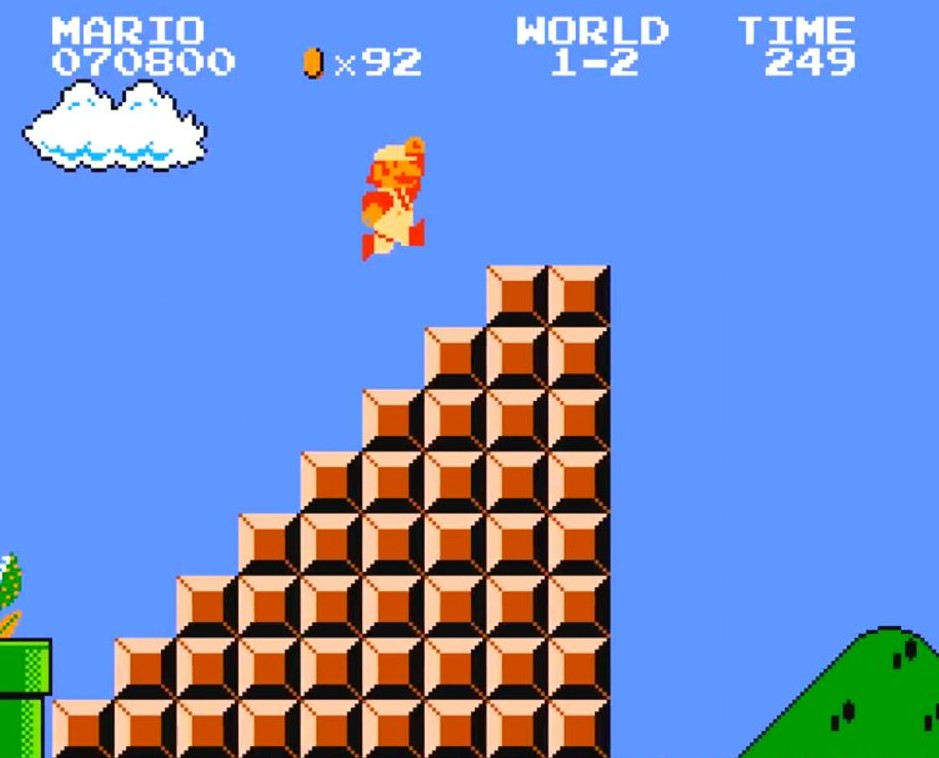
\includegraphics[width=\textwidth]{pages/img/SuperMarioBros.jpg}
        \caption{Super Mario Bros (1985).}
        \label{fig:super_mario_bros}
    \end{subfigure}
    \hfill
    % Subfigura derecha (Pac-Man)
    \begin{subfigure}[b]{0.45\textwidth}
        \centering
        
\includegraphics[width=\textwidth]{pages/img/Sonic.png}
        \caption{Sonic The Hedgehog (1991).}
        \label{fig:sonic}
    \end{subfigure}
    \caption{Títulos pioneros orientados a la superación de puntuaciones en la época arcade.}
    \label{fig:plataformas}
\end{figure}
    
    \item \textbf{Aventuras y Juegos de Rol (RPG):} Los primeros juegos de aventura nacieron como experiencias basadas en texto, siendo \textit{Colossal Cave Adventure} (1976)\cite{colossal_cave}  el pionero en fundar el género mediante la resolución de acertijos en pantallas interactivas, lo que más tarde derivó en las aventuras gráficas de los 80 y 90. En paralelo, los RPG digitalizaron los sistemas de los juegos de rol de mesa. Ambos géneros rompieron con la linealidad de los niveles estáticos para ofrecer mundos interconectados enfocados en la exploración y la narrativa; para lograrlo, los RPG de la época estandarizaron la perspectiva cenital (\textit{Top-Down}) como la herramienta visual óptima para gestionar el espacio y mejorar la experiencia del usuario.
\end{itemize}

\subsection{La historia reciente y la diversificación de subgéneros}

Con el paso de los años, la evolución tecnológica y la creatividad que los diseñadores impregnaban en cada título —en producciones donde las barreras creativas parecían disolverse— provocaron la ramificación de los géneros de videojuegos en un sinfín de subgéneros. Estas variantes nacían tanto de cambios radicales en la jugabilidad dentro de un mismo género, como de configuraciones concretas de la cámara o modificaciones sutiles de sus mecánicas básicas.

En la última década, este fenómeno de hiperespecialización se ha visto acelerado exponencialmente por la democratización de motores gráficos comerciales y herramientas de desarrollo accesibles. Esta apertura tecnológica propició el denominado "boom indie" (desarrollo independiente), un ecosistema donde estudios de menor tamaño, liberados de las rígidas exigencias comerciales de las grandes superproducciones (mercado AAA), comenzaron a deconstruir y experimentar con las convenciones clásicas del medio.

Como resultado, la industria contemporánea se caracteriza profundamente por la hibridación mecánica. Las fronteras estrictas que durante los años noventa separaban la acción, la estrategia o la aventura se han difuminado para dar paso a la integración de sistemas complejos. Conceptos modernos como el \textit{Roguelite} (generación procedimental con progresión permanente) o el \textit{Soulslike} (énfasis en el castigo por el error, la gestión meticulosa de la resistencia y la narrativa ambiental) han permeado en la inmensa mayoría de las categorías tradicionales. Los jugadores actuales ya no buscan experiencias unidimensionales, sino propuestas que combinen capas de diferentes géneros para generar nuevas dinámicas de juego.

Dentro de este panorama reciente, los dos géneros que vertebran este proyecto han sufrido redefiniciones fundamentales:

\begin{itemize}
    \item Por un lado, las aventuras en perspectiva cenital (\textit{Top-Down}) han trascendido la simple exploración lineal o el combate básico (\textit{Hack and Slash}). En la actualidad, estos entornos bidimensionales se utilizan frecuentemente para enmarcar experiencias de supervivencia (\textit{Survival Horror}), donde el control de una cámara limitada se aprovecha para generar puntos ciegos y tensión psicológica. La jugabilidad contemporánea en estos subgéneros exige la gestión táctica de recursos muy escasos y el enfrentamiento contra inteligencias artificiales que obligan al jugador a medir cada enfrentamiento.
    \item Por otro lado, el género de plataformas ha vivido un renacimiento técnico y de diseño a través de su variante más extrema: el plataformas de precisión (\textit{Precision Platformer}). Obras referentes de los últimos diez años han optado por eliminar por completo las penalizaciones tradicionales (como el sistema de vidas limitadas o los tiempos de carga tras morir), apostando por la reaparición instantánea. Este cambio de paradigma enfoca la experiencia en el ensayo y error a gran velocidad, exigiendo al usuario un dominio casi coreográfico de mecánicas de movilidad avanzada, como el salto rebotado (\textit{Wall Jump}), el deslizamiento y el impulso aéreo (\textit{Dash}).
\end{itemize}

Paralelamente a esta evolución mecánica, la historia reciente del videojuego ha consolidado el uso de la estética \textit{Pixel Art}. Lejos de ser una limitación impuesta por el hardware como en sus orígenes, en la actualidad se trata de una decisión artística y nostálgica deliberada que busca evocar la época dorada de las consolas de 16 bits. \textit{Reset} se enmarca exactamente en este contexto de diseño moderno: utiliza el estilo visual retro para apelar a la memoria histórica del jugador, pero aplica una arquitectura de hibridación de subgéneros y mejoras de calidad de vida (\textit{Quality of Life}) para ofrecer una experiencia de juego adaptada a los exigentes estándares de fluidez (\textit{Game Feel}) contemporáneos.

Esas ramificaciones se han ido completando hasta crear un árbol de dimensiones y complejidad casi incomprensibles para la mayoría de jugadores casuales. Ese es uno de los pilares que se tratan en \textit{Reset}, que recoge esta herencia histórica y asume la complejidad técnica de difuminar dichas fronteras, integrando en una sola arquitectura las diversas mecánicas y configuraciones jugables analizadas.

\subsection{Justificación de la arquitectura de diseño en RESET: Modelos de hibridación por paradigmas}

El desarrollo de un proyecto de software interactivo de forma unipersonal exige una planificación rigurosa que optimice los recursos técnicos sin sacrificar la profundidad de la experiencia de usuario. En este contexto, \textit{Reset} se estructura formalmente a través de dos paradigmas jugables bien diferenciados, distribuidos en mundos independientes. Esta segmentación no solo divide la carga del diseño de niveles (\textit{Level Design}), sino que sirve para demostrar cómo filosofías de juego propias de grandes producciones contemporáneas en tres dimensiones (como la tensión de \textit{Resident Evil} \cite{resident_evil_game} o las dinámicas de aventura de \textit{The Last of Us} \cite{last_of_us_game}) pueden ser deconstruidas y trasladadas con éxito a un entorno bidimensional optimizado bajo la perspectiva \textit{Top-Down} y el formato de desplazamiento lateral.

\subsubsection{Paradigma 1: La Aventura Cenital y la adaptación del Survival Horror}

El primer bloque del proyecto articula la convergencia entre la exploración clásica y la tensión psicológica, estructurando la experiencia en dos subgéneros claramente diferenciados que representan distintas evoluciones de la vista cenital. 

Para el primer nivel, el diseño se decanta hacia la acción-aventura con un enfoque directo en el combate (\textit{Hack and Slash}). La base del sistema de enfrentamiento cuerpo a cuerpo y el tránsito espacial se fundamenta en los estándares establecidos por títulos como \textit{The Legend of Zelda: A Link to the Past} (1991)\cite{zelda_alttp} (ver Figura~\ref{fig:zelda}), que demostró la viabilidad de la interacción táctica en espacios bidimensionales. En esta fase, la jugabilidad prioriza la agilidad en la exploración de las diversas zonas y el combate directo contra los enemigos, sirviendo como una primera toma de contacto centrada en el dinamismo y la acción mecánica.

\begin{figure}[H]
    \centering
    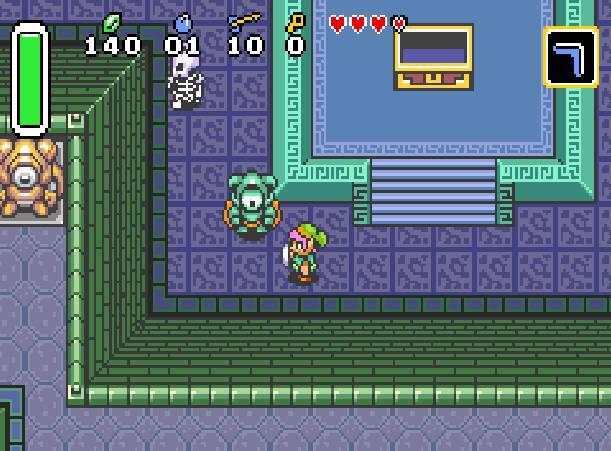
\includegraphics[width=0.45\textwidth]{pages/img/LegendOfZelda.jpg}
    \caption{The Legend of Zelda: A Link to the Past (1991).}
    \label{fig:zelda}
\end{figure}

Sin embargo, en el segundo nivel de este mundo, \textit{Reset} altera la naturaleza ágil de la aventura clásica al inyectarle las mecánicas sistémicas del \textit{Survival Horror} puro. La dinámica cambia por completo al introducir el combate a distancia, obligando al jugador a explorar exhaustivamente los escenarios en busca de notas, objetos clave y contraseñas para poder resolver los puzles que bloquean el avance. 

Para lograrlo, se toma como referencia la atmósfera opresiva y la escasez de recursos de obras referentes de la supervivencia como \textit{The Last of Us}, combinándolo con la implementación técnica de un inventario matricial limitado por cuadrículas característico de la saga \textit{Resident Evil}. Esta decisión de diseño traslada la toma de decisiones estratégicas al jugador, quien debe evaluar el coste de cada enfrentamiento y decidir si emplear su valiosa munición o recurrir a la evasión. Casos de estudio modernos como \textit{Signalis} (2022)\cite{signalis_game} o el enfoque bidimensional de \textit{Lone Survivor} (2012)\cite{lone_survivor} (ver Figura~\ref{fig:SurvivalHorrors}) validan esta metodología, demostrando que la vulnerabilidad del avatar, la restricción de visibilidad y la atmósfera opresiva no dependen de una tecnología tridimensional, sino de la coherencia en la aplicación de las reglas lúdicas dentro de un entorno \textit{Pixel Art}.

\begin{figure}[H]
    \centering
    % Subfigura izquierda (Space Invaders)
    \begin{subfigure}[b]{0.45\textwidth}
        \centering
        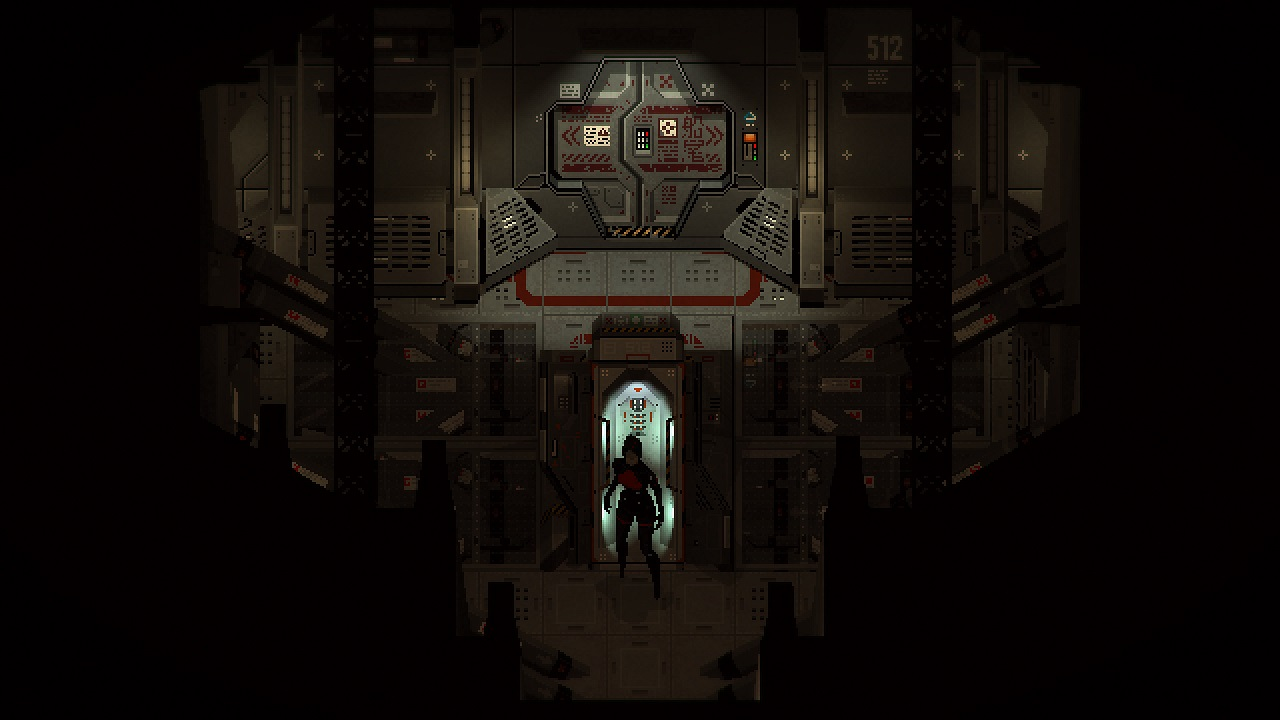
\includegraphics[width=\textwidth]{pages/img/Signalis.jpg}
        \caption{Signalis (2022).}
        \label{fig:signalis}
    \end{subfigure}
    \hfill
    % Subfigura derecha (Pac-Man)
    \begin{subfigure}[b]{0.45\textwidth}
        \centering
        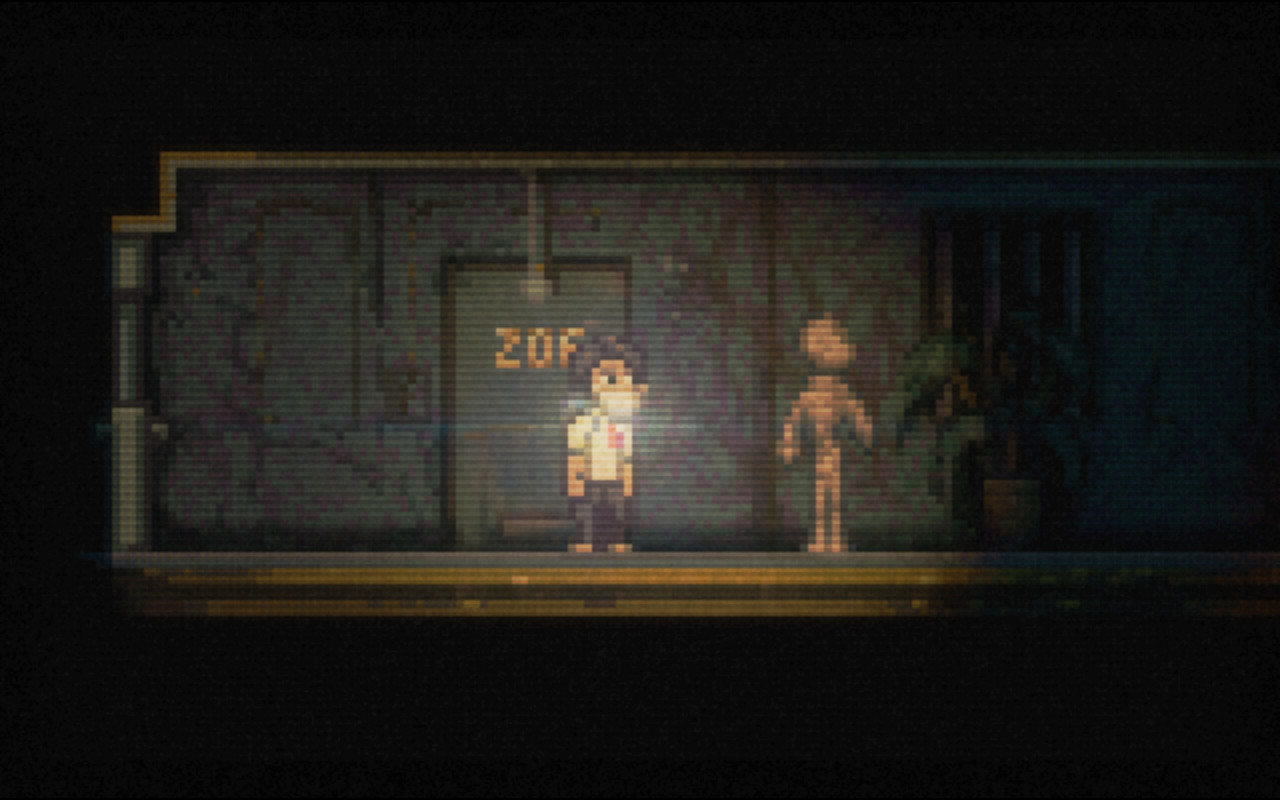
\includegraphics[width=\textwidth]{pages/img/LoneSurvivor.jpg}
        \caption{Lone Survivor (2012).}
        \label{fig:sonic}
    \end{subfigure}
    \caption{Títulos pixel art actuales de survival horror}
    \label{fig:SurvivalHorrors}
\end{figure}

\subsubsection{Paradigma 2: Del Plataformas Clásico a la Hiperespecialización de Precisión}

El segundo entorno del juego aborda una transición pedagógica y técnica sobre la evolución de la movilidad del personaje, dividiendo la experiencia en dos niveles de dificultad orgánica:

\begin{itemize}
    \item \textbf{El Plataformas Clásico:} Configurado como un entorno introductorio permisivo con el usuario, utiliza como marco de estudio obras como \textit{Super Mario World} (1990) (ver Figura~\ref{fig:marioworld}). En esta fase, el diseño del código prioriza el control intuitivo de la inercia, la parábola física del salto y la eliminación de amenazas mediante la colisión vertical del avatar sobre los enemigos, asentando una base accesible de control del espacio.

\begin{figure}[H]
    \centering
    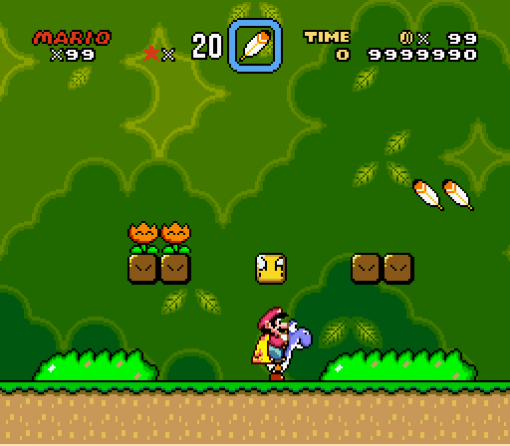
\includegraphics[width=0.45\textwidth]{pages/img/MarioWorld.png}
    \caption{Super Mario World (1991).}
    \label{fig:marioworld}
\end{figure}
    
    \item \textbf{El Plataformas de Precisión:} Concebido como el pico de dificultad técnica del proyecto, este nivel evoluciona hacia el formato del \textit{Precision Platformer}. Se toman como pilares fundamentales de diseño \textit{Super Meat Boy} (2010)\cite{super_meat_boy} (ver Figura~\ref{fig:meatboy}), por su aproximación al bucle rápido de ensayo y error frenético, y \textit{Celeste} (2018)\cite{celeste_game} (ver Figura~\ref{fig:celeste}), del cual se realiza una traslación directa de mecánicas avanzadas. El motor de \textit{Reset} replica de este último el impulso aéreo en las diferentes direcciones (\textit{Dash}), el deslizamiento y agarre a superficies verticales (\textit{Wall Slide}) con su correspondiente impulso (\textit{Wall Jump}) y el impulso extra en el aire en forma de salto (\textit{Double Jump}). Estructuralmente, destaca la fragmentación del escenario en micro-retos independientes contenidos en zonas marcadas. Este enfoque técnico elimina los sistemas arcaicos de penalización por vidas limitadas, reenfocando la frustración lúdica del usuario hacia la ejecución coreográfica y precisa de los controles.

\begin{figure}[H]
    \centering
    % Subfigura izquierda (Space Invaders)
    \begin{subfigure}[b]{0.45\textwidth}
        \centering
        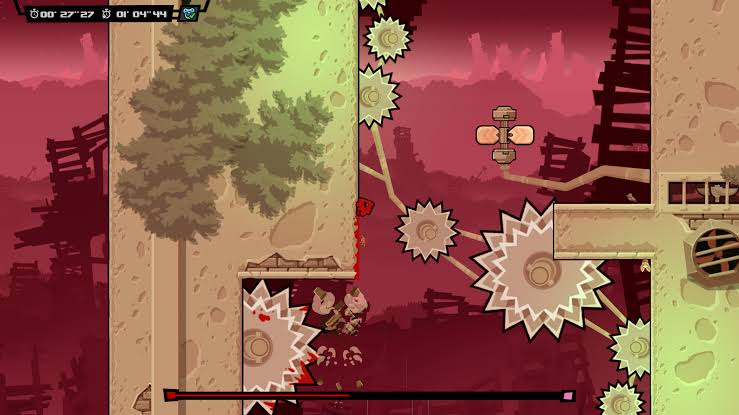
\includegraphics[width=\textwidth]{pages/img/SuperMeatBoy.jpg}
        \caption{Super Meat Boy (2010).}
        \label{fig:meatboy}
    \end{subfigure}
    \hfill
    % Subfigura derecha (Pac-Man)
    \begin{subfigure}[b]{0.45\textwidth}
        \centering
        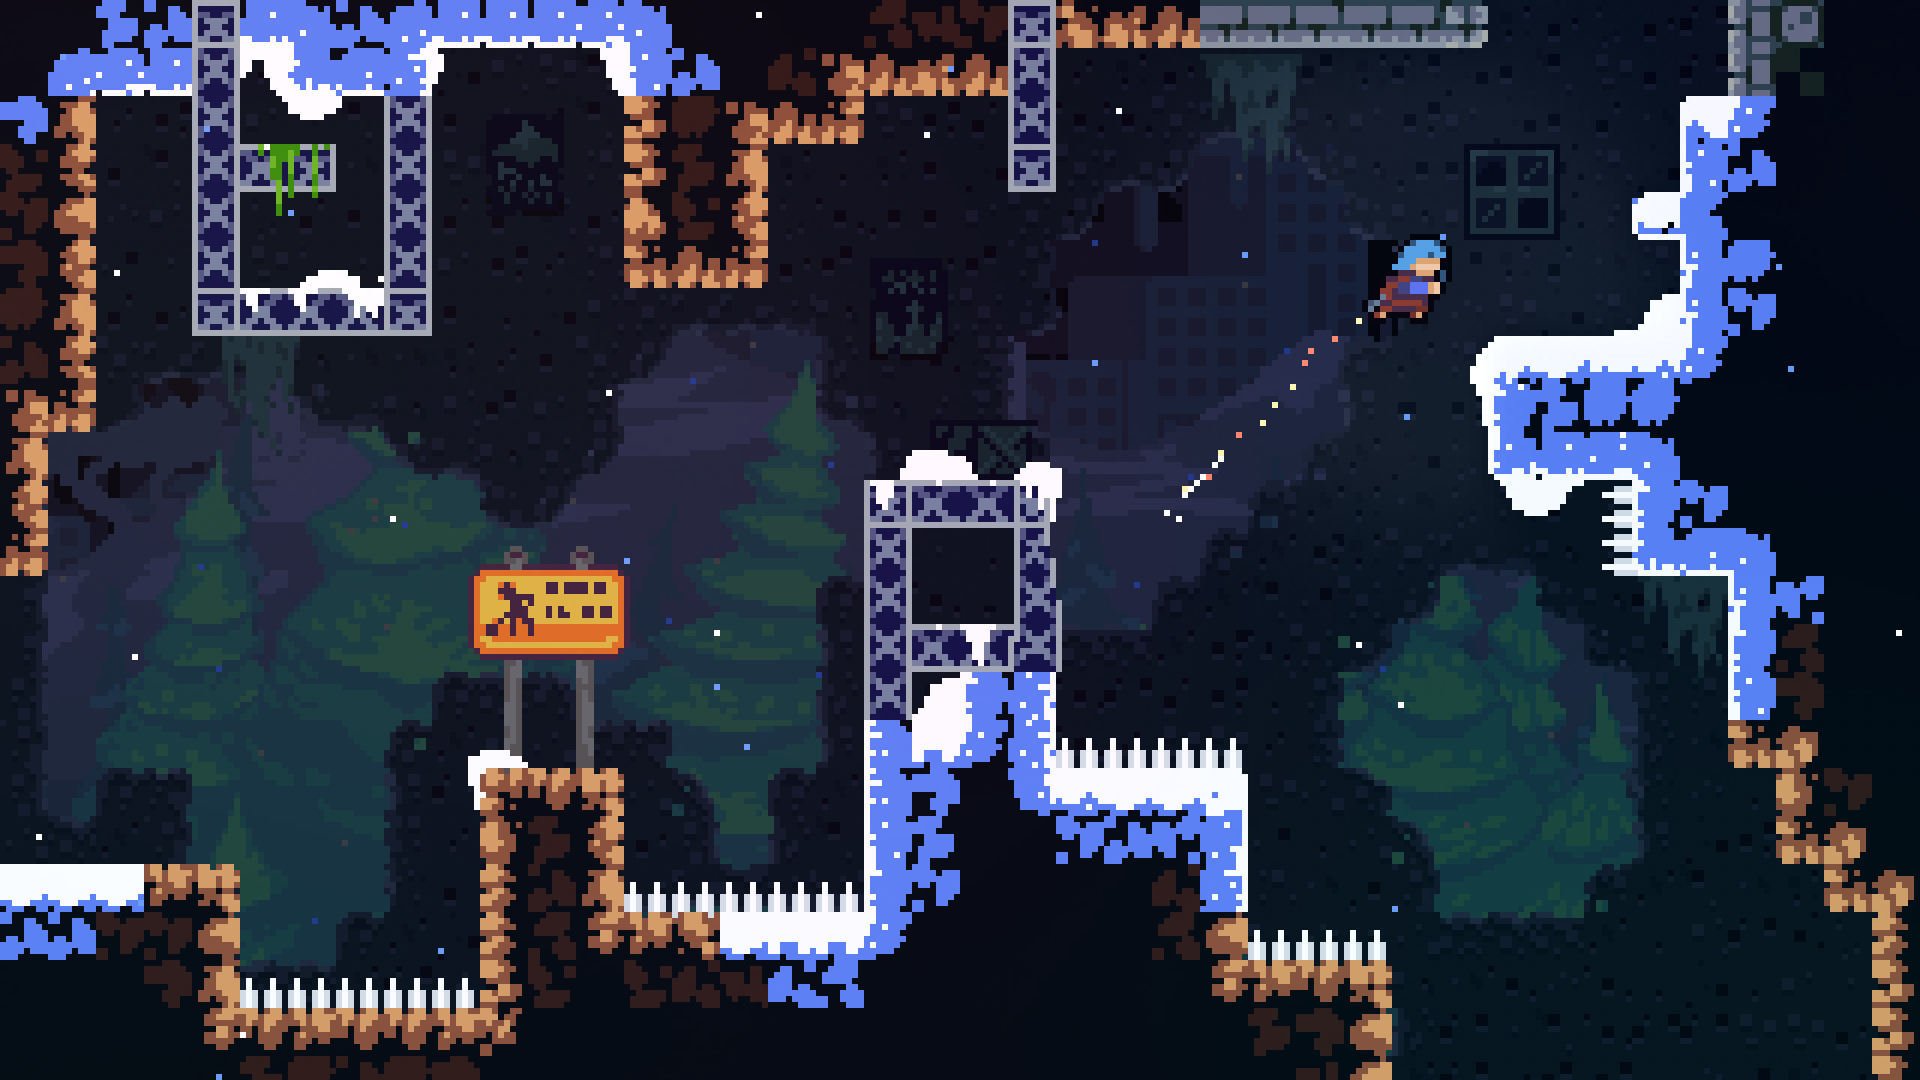
\includegraphics[width=\textwidth]{pages/img/Celeste.jpg}
        \caption{Celeste (2018).}
        \label{fig:celeste}
    \end{subfigure}
    \caption{Títulos pixel art actuales de plataformas}
    \label{fig:PlataformasParkour}
\end{figure}
\end{itemize}